\section{Convex Hull}\label{sec:ch}
Another commonly used compactness score is the \textit{convex hull
score}.  We briefly recall the definition of a convex set and then
define this score function.

\begin{definition}
  A set $X$ in a metric space is \textbf{convex} if for any pair of
  points $x_1$ and $x_2$ in $X$, the shortest geodesic segment
  connecting $x_1$ and $x_2$ is entirely contained in $X$. 
\end{definition}
In the plane, these geodesic segments are ordinary line segments.  On
the sphere, the geodesics are segments of great circles. In 
particular, this means that on the sphere, caps are 
convex, and in the plane, circular regions are convex.

\begin{definition}
  Let $\mathrm{conv}(\Omega)$ denote the \textit{convex hull} of
  a region $\Omega$ in either the sphere or the plane, which is the
  smallest convex region containing $\Omega$.  Then we define the
  \textit{convex hull score} of $\Omega$ as 
  \begin{align*}
    \mathrm{CH}(\Omega)=
    \frac{\mathrm{area}(\Omega)}{\mathrm{area}(\mathrm{conv}(\Omega))}
  \end{align*}
\end{definition}

The convex hull score of a region $\Omega$  will be equal to one if
and only if $\Omega$ is itself convex.  We note that the convex hull
and Polsby-Popper scores agree when $\Omega$ is a circle, provide
a similar score when $\Omega$ is roughly circluar, and differ greatly
if $\Omega$ is a highly non-circular but convex region, such as
a long, thin rectangle.

Our strategy to demonstrate that any map projection cannot preserve
the orders of convex hull scores will be similar to the previous
section. We first argue that any order-preserving map must, in
particular, preserve the maximizers in the ordering, meaning convex
regions on the sphere are mapped to convex regions in the plane.
Then, we use this condition to restrict our attention to the map
projections which preserve these maximizers, which we can then use to
construct our counterexample.

\abn{muted some stuff... Let the theorems speak for themselves?}
\mute{
An overview of the structure of the argument is as follows:
\begin{enumerate}
  \item Any map projection which preserves the ordering of convex
    hull scores must, in particular, preserve the maximizers in that
    ordering.  This means that such a projection must send convex
    sets on the sphere to convex sets in the plane.
  \item One projection which is convexity-preserving is the gnomonic
    projection.
  \item Affine linear transformations of the plane are also
    convexity-preserving.
  \item \textit{Any} map projection which is convexity-preserving
    must be the composition of the gnomonic projection and an affine
    linear transformation.
  \item The gnomonic projection does not preserve the ordering of
    convex hull scores, and any affine linear transformation
    \textit{does}.
  \item Therefore, there is no composition of the gnomonic
    projection and an affine linear projection which together
    preserve the ordering of convex hull scores.
\end{enumerate}

Since the convex hull score of $\Omega$ is one if and only if $\Omega$
is itself a convex region, the maximizers of the induced score
ordering are exactly the convex sets in the surface of interest. We
can observe that if there is some map projection which preserves the
ordering of convex hull scores, it must at the very least map convex
sets in the sphere to convex sets in the plane (and vice versa), since
convex sets are the maximizers of the convex hull score.

As it turns out, the family of map projections which send every convex
set on the lower half-sphere to a convex set in the plane is exactly
the set of projections which can be written as a composition of the
\textit{gnomonic projection} from the lower half-sphere to the plane
followed by an \textit{affine linear transformation}.
}

\begin{definition}
  The \textbf{gnomonic projection} is the map projection from the
  lower half-sphere to the plane defined by placing the south pole of
  the sphere tangent to the plane at the origin and sending a point
  $p$ on the lower half-sphere to the unique point $q$ in the plane
  which lies on the line in $\mathbb{R}^3$ which passes through the
  center of the sphere, $p$ and $q$.
\end{definition}
By convention, we will let the sphere be the unit sphere 
centered at $(0,0,1)$.

Intuitively, the image of a region on the sphere under the gnomonic
projection is the shadow in the plane of that region which is
created when we put the bottom of the sphere at the origin and turn
on a light source at the center of the sphere.

\zs{do we want to write the explicit parametrization of the gnomonic
projection here? the xy version of it is pretty gross.  the polar
version is less messy.  I don't know if it provides any extra
insight...}

We can observe that the gnomonic projection sends caps centered at the
south pole to circles in the plane centered at the origin, and sends
any segment of a great circle passing through the south pole to a line
segment in the plane passing through the origin.  What may be somewhat
surprising is that it sends \textit{every} convex set on the sphere to
a convex set in the plane.

\begin{lemma} \label{lem:gnomonic_convex}
  Let $\vphi$ be the gnomonic projection, and $U\subset S^2$ a convex 
  set. Then $\vphi(U)$ is convex.
\end{lemma}
\begin{proof}
  To prove this, it suffices to show that the one-dimensional convex
  sets are preserved. In other words, we must show that any segment of 
  a great circle on the sphere is sent to a line segment in the plane.

  Let $p$ be the center of the sphere $S^2$, and let $C\subset S^2$ be
  a geogesic segment in the lower hemisphere.  Note that $C$ is uniquely
  identified by the intersection of $S^2$ with a portion of a hyperplane
  $\mc{P}$ passing through $p$, and not parallel to the $xy$-plane,
  $\mc{P}_{xy}$. By construction, $\vphi(C)\subset \mc{P}\cap
  \mc{P}_{xy}$, which is a line. 

  Since the gnomonic projection is injective, it follows that 
  geodesic segments in $S^2$ cannot be sent to points, and hence 
  must be sent to lines.

  \mute{
  Then, for any point $p$ on the
  great circle, the line passing through the sphere's center and $p$ is
  contained within this plane.  But this is exactly the construction
  used to find the image of $p$ under the projection, so if $p$ is
  mapped to the point $q$, then $q$ is also on this line and therefore
  in the plane, and $q$ must lie at the intersection of the slicing
  plane and the projection plane.  Since the intersection of two planes
  is a line, any choice of $p$ on the great circle is sent to a $q$ on
  this line of intersection, so the image of any segment of the great
  circle is a segment of a line.
  }
\end{proof}

\abn{I'm still hunting down the reference for this theorem. 
Some say it's due to Hartshorne, but I can't find the reference. 
Someone says it's due to von Staudt from the 1850's...}
\begin{theorem} \label{thm:geometric_algebra}
  If $f:\R^n\supset U\to\R^n$ is injective, sends straight 
  lines to straight lines, and $n>1$, then $f$ is an affine linear 
  transformation.
\end{theorem}
\begin{proof}
  After possibly translating, we can assume that 
  $0\in U$ and $f(0) = 0$, in which 
  case we must show that $f$ is linear. We write $V = f(U)$. 
  Since $f$ is a bijection from $U$ to $V$ 
  sending straight lines to straight lines, it follows that 
  if $\mc{P}$ is an affine subspace of $\R^n$, then 
  $f(\mc{P}\cap U)$ must be of the form $\mc{Q}\cap V$, where 
  $\mc{Q}$ is an affine subspace of $\R^n$.
  Additionally, $f$ must preserve intersections of 
  lines, and hence sends coplanar parallel lines to coplanar 
  parallel lines, and hence nondegenerate parallelograms 
  to nondegenerate parallelograms.

  Let $v\in U$ be some nonzero vector, and let 
  $w\in U\ssm \mathrm{Span}(v)$ be such that 
  $v+w\in U$.
  Restricted to the plane $\mathrm{Span}(v,w)$, 
  we can draw the following parallelogram:
  \begin{figure}
    \centering
    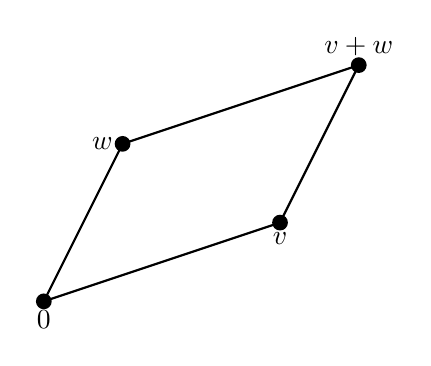
\begin{tikzpicture}[scale=1pt]
      \draw[thick] (0,0) -- (3,1) node[below] {};
      \draw[thick] (0,0) -- (1,2) node[left] {};
      \draw[thick] (1,2) -- (4,3) node[above] {};
      \draw[thick] (3,1) -- (4,3) node[right] {};
      \fill (3,1) circle (0.1) node[below] {$v$};
      \fill (1,2) circle (0.1) node[left] {$w$};
      \fill (0,0) circle (0.1) node[below] {$0$};
      \fill (4,3) circle (0.1) node[above] {$v+w$};
    \end{tikzpicture}
  \end{figure}
  By the above discussion, $f$ sends this parallelogram 
  to another parallelogram whose vertices are 
  $0$, $f(v)$, $f(w)$, and $f(v+w)$. By the geometric 
  interpretation of vector addition, this means that 
  $f(v+w) = f(v)+f(w)$. A similar argument works for 
  subtraction.

  Now, if $w\in \mathrm{Span}(v)\cap U$, then choose some 
  $u\in U\ssm \mathrm{Span}(v)$, and apply the above argument to 
  the pair $w-u$ and $v+u$, and then to the pairs 
  $w,u$ and $v,u$ to get $f(v+w) = f(v) + f(w)$.

  Let $v\in U\ssm \{0\}$ and $\alpha \in \R\ssm 0$ be such that 
  $\alpha v\in U$. We can write $f(\alpha v) = g(\alpha,v)f(v)$, and
  we need to show that $g$ does not depend on $v$. Let
  $w\in U\ssm \mathrm{Span}(v)$ be such that $\alpha w\in U$, 
  and consider the following line configuration:
  \begin{figure}
    \centering
    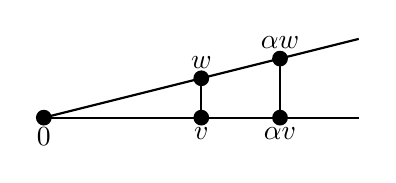
\begin{tikzpicture}
      \draw[thick] (0,0) -- (4,0) node[below] {};
      \draw[thick] (0,0) -- (4,1) node[left] {};
      \draw[thick] (2,0) -- (2,0.5) node[above] {};
      \draw[thick] (3,0) -- (3,0.75) node[above] {};
      \fill (0,0) circle (0.1) node[below] {$0$};
      \fill (2,0.5) circle (0.1) node[above] {$w$};
      \fill (2,0) circle (0.1) node[below] {$v$};
      \fill (3,0.75) circle (0.1) node[above] {$\alpha w$};
      \fill (3,0) circle (0.1) node[below] {$\alpha v$};
    \end{tikzpicture}
  \end{figure}
  Where the lines $(v,w)$ and $(\alpha v,\alpha w)$ are parallel. 
  Since $f$ preserves line configurations and paralellism, if 
  $f(\alpha v) = \beta f(v)$, then 
  $f(\alpha w) = \beta f(w)$. The case when 
  $w\in \mathrm{Span}(v)$ is treated similarly to additivity. 
  Overall, we get that $g$ as defined above 
  does not depend on $v$.

  Morevoer, it is easy to check that $g$ wherever 
  $g$ is defined, $g(\alpha+\beta) = g(\alpha) + g(\beta)$ 
  and $g(\alpha\beta) = g(\alpha)g(\beta)$, and hence 
  is a restriction of a field 
  automorphism of $\R$, and hence is the identity.
\end{proof}
Note that we have actually proved a stronger result 
for a general field:
\begin{theorem}
  Let $\K$ be a field with at least three elements, and 
  let let $n>1$. Let $f:\K^n\to \K^n$ be a bijection. Then 
  there exists $z\in \K^n$ such that for all 
  $x,y\in \K^n$ and $\alpha\in \K$,
  \begin{align*}
    f(\alpha x) = g(\alpha)f(x) + f(y) + z
  \end{align*}
  Where $g:\K\to\K$ is a field automorphism.

  Such a function is called \textit{semilinear}
\end{theorem}
We can prove this by taking $U = \K^n$ and following the same argument. 
The condition $|\K|\ge 3$ is to be able to characterize 
parallel lines as disjoint lines lying in the same affine plane.

Using this, we can complete the construction of the main tool of this
section -- that any map projection which preserves convex sets can be
written as the composition of the gnomonic projection and an affine
linear transformation of the plane.

\begin{theorem}
  Let $\psi:U\to \R^2$ be a map projection 
  defined on the lower-hemisphere, and let 
  $\vphi$ be the gnomonic projection. If $\psi^{-1}$ sends 
  convex sets to convex sets, then there exists an affine linear map 
  $L$ such that $\psi = L\circ \vphi$.
\end{theorem}

\begin{proof}
  By Lemma ~\ref{lem:gnomonic_convex}, the map $\vphi\circ
  \psi^{-1}:\psi(U)\to \R^2$ sends convex sets to convex sets. It is
  bijective, since $\psi$ and $\vphi$ are bijective, and hence
  satisfies the conditions of Theorem ~\ref{thm:geometric_algebra}, 
  meaning that there exists an affine linear isomorphism 
  $L^{-1}:\R^2\to \R^2$ such that $\vphi = \psi \circ L^{-1}$. 
  Thus, $\psi = \vphi \circ L$, as desired.
  \mute{
  By the previous lemma, the gnomonic projection does indeed preserve
  convex sets.   If a map projection preserves convex sets, it must in
  particular preserve the one-dimensional convex sets, meaning it maps
  segments of great circles on the sphere to line segments in the
  plane.  Take $\psi$ and $\varphi$ to convexity-preserving map
  projections, and, without loss of generality take $\varphi$ to be
  the standard gnomonic projection described above. We consider the
  composition $\psi\varphi^{-1}$, which is a transformation of the
  plane which preserves convex sets, so in particular it sends line
  segments to line segments.  Since these transformations also
  preserve containment, we can additionally observe that
  $\psi\varphi^{-1}$ preserves \textit{collinearity} in the plane,
  which means it is an affine linear transformation of the plane.
  Since we can write $\psi$ as $\psi\varphi^{-1}\varphi$, we have
  successfully written our convexity-preserving map as the composition
  of the gnomonic projection and an affine linear transformation of
  the plane.}
\end{proof}
We now show that the gnomonic projection does not preserve 
convex-hull score orderings.

\abn{mute this and write it in later:
This lemma lets us prove our theorem in two steps.  We can first show
that the gnomonic projection does not preserve the ordering of convex
hull scores, then argue that this misordering cannot be corrected by
any affine linear transformation of the plane.  This first part we
will prove by explicitly constructing two regions whose convex hull
scores are permuted under the gnomonic projection, and to facilitate
this construction, we make the following observation:
}
\abn{Condensed all of this to one paragraph. See below.
\begin{example}
  Let $\varphi$ be the gnomonic projection and $C_\theta$ be a spherical
  cap centered at the south pole parametrized by the angle $\theta$
  formed between the central axis of the sphere and a line segment
  between the center of the sphere and the boundary of the cap. 
  Then $\varphi(C_\theta)$ is a disk in the
  plane, centered at the origin, and has radius $\tan(\theta)$.

  \begin{figure}
    \centering
    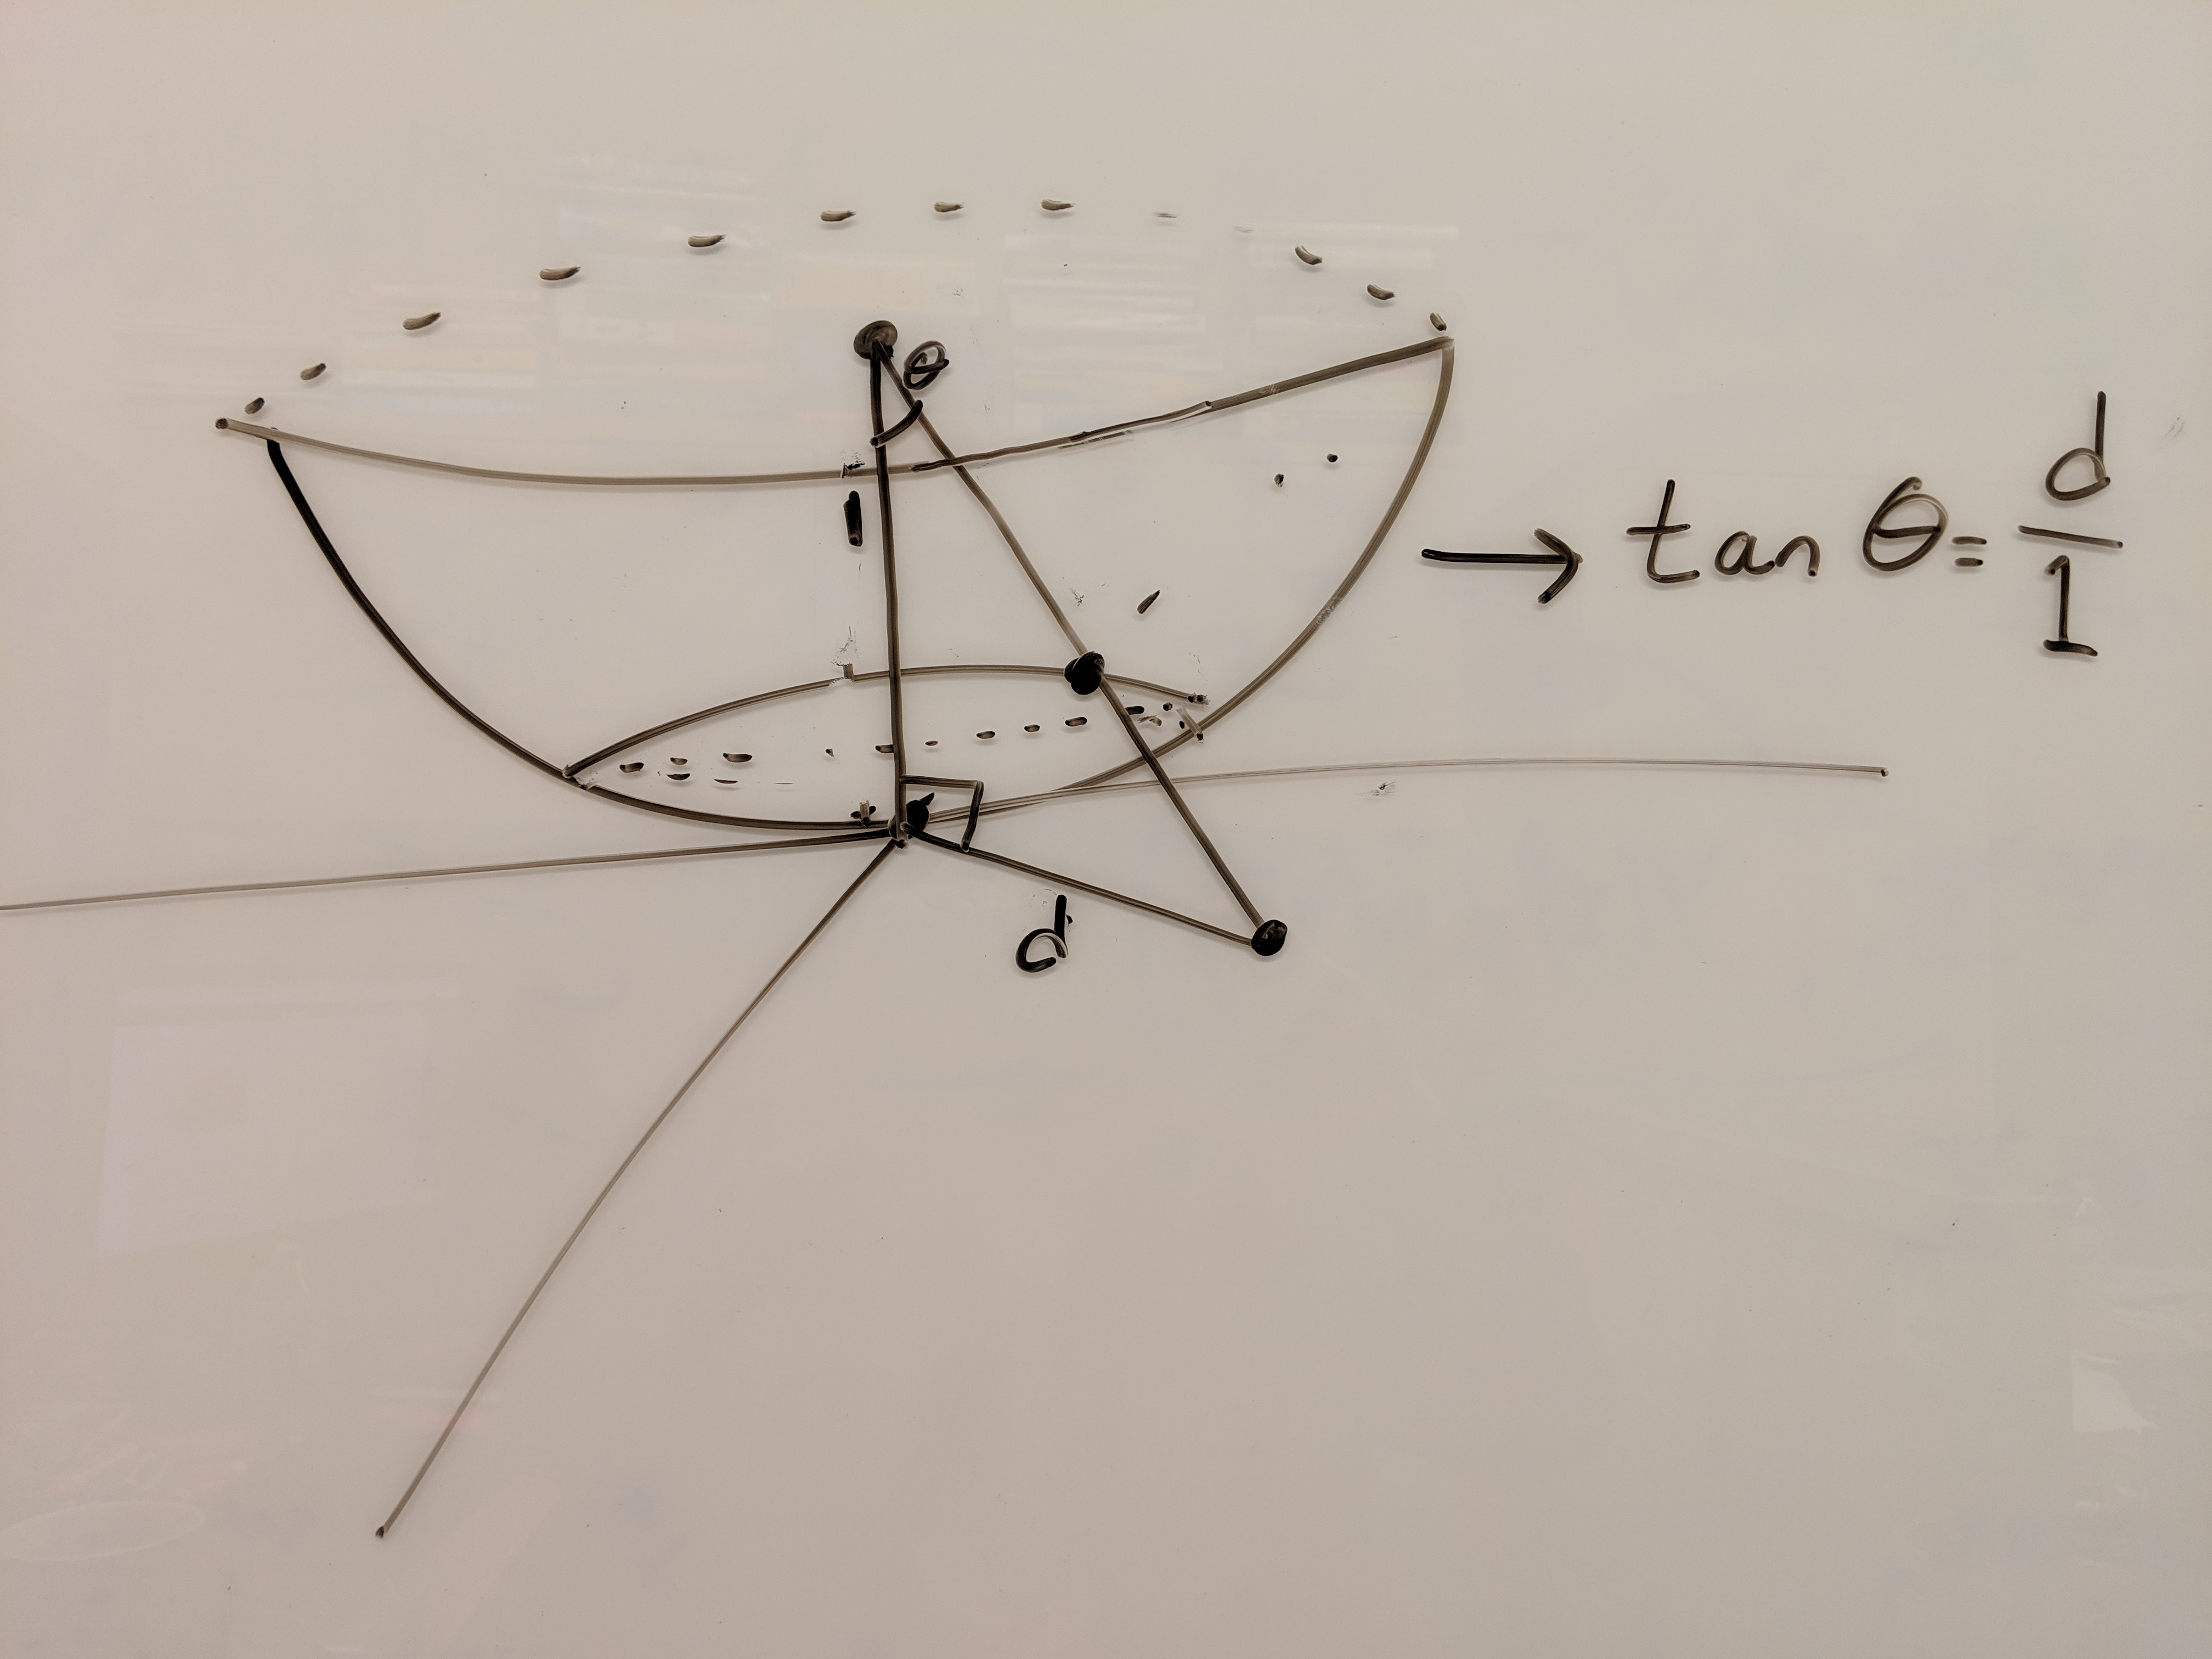
\includegraphics[width=.8\textwidth]{figs/gnom_cap.jpg}\\
    \caption{The image of a cap with polar angle $\theta$ is a circle of radius $\tan\theta$.}
    \label{fig:gnomcap}
  \end{figure}

  \begin{proof}

    A (literal) sketch of this proof can be seen in Figure~\ref{fig:gnomcap}.

    Since $\varphi$ projects from the center of the sphere and the
    sphere's south pole is mapped to the origin in the plane, the
    image of $C_\theta$ is totally radially symmetric about the
    origin, and is therefore a circle.  To see that its radius is
    $\tan(\theta)$, place the south pole of the sphere tangent to the
    plane at the origin. By construction, for any point $p$ on the
    boundary of $C_\theta$, there is a unique line passing through the
    center of the sphere, $p$, and the point $\varphi(p)$ on the
    boundary of the disk in the plane.  By definition, this line meets
    the central axis of the sphere at an angle of $\theta$, and the
    central axis of the sphere meets the plane orthogonally, so the
    center of the sphere, the origin, and the point $\varphi(p)$ form
    a right triangle with angle $\theta$.  Since we know that the
    distance between the center of the sphere and the origin is 1, we
    can write the distance between the origin and $\varphi(p)$ as
    $\tan(\theta)$.
  \end{proof}
  Using this, we can perform the construction of two regions whose
  convex hull scores are permuted by the gnomonic projection.

  \begin{lemma}
    There exist two regions on the sphere, $A$ and $B$, such that
    $\mathrm{CH}(A) > \mathrm{CH}(B)$ in the sphere, but, under the
    gnomonic projection $\varphi$,
    $\mathrm{CH}(\varphi(A))<\mathrm{CH}(\varphi(B))$.
  \end{lemma}

  Let $A$ be the region on the sphere defined by taking a cap centered
  at the south pole parametrized by the angle $\alpha_2$ and removing
  the cap centered at the south pole parametrized by the angle
  $\alpha_1$, with $\alpha_1<\alpha_2$.  Similarly, let $B$ be the
  region defined by angles $\beta_1$ and $\beta_2$.  The convex hull
  score of this kind of region on the sphere is $1-\frac{\text{area of
  inner cap}}{\text{area of outer cap}}$.  The projection under
  $\varphi$ of this kind of region is a disk in the plane with
  a smaller, cocentric disk deleted.  The convex hull score of this kind
  of region in the plane is $1-\frac{\text{area of inner
  disk}}{\text{area of outer disk}}$.  

  In the previous section, we parametrized a cap on the sphere by its
  \textit{height}, but we can instead parametrize it by its
  \textit{polar angle}, which is the angle formed between the polar axis
  and a line segment connecting the center of the sphere with the
  boundary of the cap.  Using the notation of $h$ for the height of
  a cap and $r$ for its radius as before, and letting $\theta$ be the
  cap's polar angle, we can use trigonometry to rewrite the area of the
  cap at height $h$, $\kappa(h)$.  Since $(1-h)=\cos(\theta)$, the area
  of the cap at height $h$ is $2\pi (1-\cos(\theta))$.  Therefore, if we
  have two cocentric caps on the disk parametrized by angles
  $\theta_1<\theta_2$, the convex hull score of this region is 

  $$1-\frac{2\pi (1-\cos(\theta_1))}{2\pi (1-\cos(\theta_2))}
  = 1-\frac{1-\cos(\theta_1)}{1-\cos(\theta_2)}.$$

  In the plane, since the image of a cap centered at the south pole
  parametrized by angle $\theta$ is a circle of radius $\tan^2(\theta)$,
  and the convex hull score of the image of a pair of cocentric caps
  parametrized by angles $\theta_1<\theta_2$ is

  $$  1-\frac{\tan^2(\theta_1)}{\tan^2(\theta_2)}.  $$

  Next, we observe that as we take a cap parametrized by an angle close
  to $\pi/2$ and increase that angle, the area of the cap grows much
  more slowly than the area of the disk defined by the cap's projection
  under $\varphi$.  This can be shown formally using
  calculus\footnote{The derivative of $1-\cos(\theta)$ is $\sin(\theta)$
  and the derivative of $\tan^2(\theta)$ is
  $2\tan(\theta)\sec^2(\theta)$.  The quantity
  $2\tan(\theta)\sec^2(\theta)-\sin(\theta)$ is positive for
  $0<\theta<\pi/2$.  We can also observe that as $\theta$ approaches
  $\pi/2$, $\tan^2(\theta)$ grows without bound, but $1-\cos(\theta)$
  approaches 1.} and intuitively recognized by considering that near
  $\theta=0$, $1-\cos(\theta)$ and $\tan^2(\theta)$ are almost equal,
  but as $\theta$ grows and approaches 1, $\tan^2(\theta)$ is much
  larger than $1-\cos(\theta)$.  What this means in the context of the
  gnomonic projection is that the areas of regions near the south pole
  of the sphere are not distorted much, but the areas of regions far
  from the south pole become very large under the projection, and
  increasingly so the further from the south pole they are. 

  We will use this observation to construct our example of two regions
  whose convex hull scores are permuted under $\varphi$, since for all
  such regions constructed as above for a fixed convex hull score on the
  sphere, those parameterized by larger angles will have comparably
  worse scores in the plane.  We will take two regions whose spherical
  convex hull scores are near $.4$, but perturbed slightly such that the
  one parametrized by larger angles has a slightly lower score.  The
  distortion of areas under the projection will more than compensate for
  this slight difference.


  Let $A$ be defined by the angles (in degrees) $\alpha_1=46^\circ$ and
  $\alpha_2=60^\circ$ and $B$ be defined by $\beta_1=20^\circ$ and
  $\beta_2=26^\circ$.  Then we have $\mathrm{CH}(A)\approx .39$ and
  $\mathrm{CH}(B)\approx .41$, but $\mathrm{CH}(\varphi(A))\approx .64$
  and $\mathrm{CH}(\varphi(B))\approx .45$, which is our example of two
  regions whose scores' order are permuted by $\varphi$.
\end{example}
}
\begin{example}
  Let $p = (0,0,1)$ be the center of the sphere, and let $0$ be the
  origin. For any angle $0\le \theta< \frac\pi2$, let $C_\theta$ be
  the spherical cap:
  \begin{align*}
    C_{\theta} = \{x|0\le\angle(x,o,p)\le \theta\}
  \end{align*}
  Let $A(\alpha_1,\alpha_2) = C_{\alpha_2}\ssm C_{\alpha_1}$ be 
  an annular region. A straightforward computation shows that:
  \begin{align*}
    \mathrm{CH}(A(\alpha_1,\alpha_2)) &= 
    1+\frac{\mathrm{Area}(C_{\alpha_1})}{\mathrm{Area}(C_{\alpha_2})}
    =1- \frac{1-\cos(\alpha_1)}{1-\cos(\alpha_2)}\\
    \mathrm{CH}(\vphi(A(\alpha_1,\alpha_2))) &=
    1+\frac{\mathrm{Area}(\vphi(C_{\alpha_1}))}%
    {\mathrm{Area}(\vphi(C_{\alpha_2}))}
      =1- \frac{\tan^2(\alpha_1)}{\tan^2(\alpha_2)}
  \end{align*}
  Where $\vphi$ is the gnomonic projection. 
  Let $A=A(\alpha_1,\alpha_2)$ be defined by the angles 
  (in degrees) $\alpha_1=46^\circ$ and
  $\alpha_2=60^\circ$ and $B=A(\beta_1,\beta_2)$ be defined by 
  $\beta_1=20^\circ$ and $\beta_2=26^\circ$. 
  Then we have $\mathrm{CH}(A)\approx .39$ and
  $\mathrm{CH}(B)\approx .41$, but $\mathrm{CH}(\varphi(A))\approx .64$
  and $\mathrm{CH}(\varphi(B))\approx .45$, which is our example of two
  regions whose scores' order are permuted by $\varphi$.
\end{example}
Now that we've shown that the gnomonic projection alone cannot
preserve convex hull scores, to complete the argument, we must now
show that there is no affine linear transformation of the plane which
can correct for this.

\begin{lemma}\label{lem:noafflin}
  Let $L$ be an affine linear transformation of the plane.  Then $L$ preserves the convex hull scores of all figures in the plane.

\end{lemma}
\begin{proof}
  Since affine linear transformations map lines to lines, they preserve
  convexity, and since they also preserve the containment of regions in
  other regions, if $\Omega$ is a region in the plane, then it must be
  the case that the convex hull of $\Omega$ is mapped to the convex hull
  of $L(\Omega)$ by $L$.  In other words, the image of the convex hull
  of $\Omega$ is the convex hull of the image of $\Omega$.  Finally,
  since affine linear transformations preserve the ratio of the areas of
  any two regions, $L$ must, in particular, preserve the ratio of the
  areas of $\Omega$ and its convex hull, so the convex hull score is
  preserved.
\end{proof}

We finally have the tools to prove the main result of this section,
which is a direct consequence of the four previous lemmas.

\begin{theorem}
  There is no map projection from the half-sphere to the plane which
  preserves the ordering of convex hull scores for all regions.
\end{theorem}

\begin{proof}
  Since such a projection must map convex regions on the sphere to
  convex regions in the plane, it must be a composition of the gnomonic
  projection followed by an affine linear transformation of the plane.
  Since affine linear transformations of the plane preserve convex hull
  scores and therefore preserve their orders, a convex hull score
  order-preserving projection from the sphere to the plane cannot exist
  if the gnomonic projection does not preserve their orders.  By the
  counterexample we constructed, it does not, and therefore there is no
  projection from the sphere to the plane which preserves the ordering
  of convex hull scores for all regions.
\end{proof}
